\documentclass[tikz,border=2pt,11pt]{standalone}
\usetikzlibrary{arrows.meta}
\usetikzlibrary{calc}
\usetikzlibrary{positioning}
\usepackage{amsmath}
\usepackage{amssymb}
\usepackage{tikz}
\usepackage{xcolor}
\newcommand{\DoNotLoadEpstopdf}{}
\begin{document}
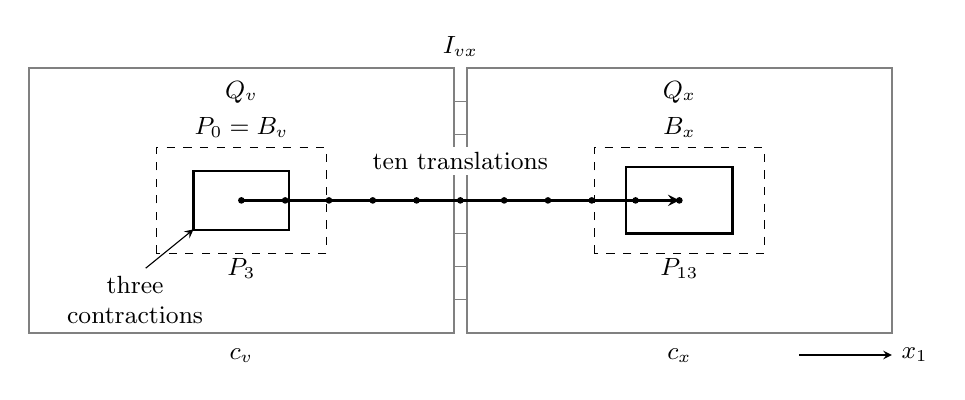
\begin{tikzpicture}[x=1.35cm,y=1.05cm,font=\small,>=stealth]
  \draw[gray,thick] (0,0) rectangle (4,3.2);
  \draw[gray,thick] (4.12,0) rectangle (8.12,3.2);
  \node at (2,2.91) {$Q_v$};
  \node at (6.12,2.91) {$Q_x$};
  \foreach \y in {0.4,0.8,1.2,1.6,2.0,2.4,2.8}{
    \draw[gray] (4,\y)--(4.12,\y);
  }
  \node[above] at (4.06,3.22) {$I_{vx}$};
  \draw[dashed] (1.2,0.96) rectangle (2.8,2.24);
  \draw[dashed] (5.32,0.96) rectangle (6.92,2.24);
  \node at (2,2.48) {$P_0=B_v$};
  \node at (6.12,2.48) {$B_x$};
  \draw[thick] (1.55,1.24) rectangle (2.45,1.96);
  \draw[thick] (5.62,1.20) rectangle (6.62,2.00);
  \node at (2,0.78) {$P_3$};
  \node at (6.12,0.78) {$P_{13}$};
  \draw[->,thick] (2,1.6)--(6.12,1.6);
  \foreach \i in {0,...,10}{
    \fill ({2+0.412*\i},1.6) circle (1.2pt);
  }
  \node[fill=white,inner sep=2pt] at (4.06,2.08) {ten translations};
  \draw[->] (1.1,0.78)--(1.55,1.25);
  \node[align=center] at (1.0,0.40) {three\\contractions};
  \node[below] at (2,-0.08) {$c_v$};
  \node[below] at (6.12,-0.08) {$c_x$};
  \draw[->] (7.25,-0.27)--(8.12,-0.27) node[right] {$x_1$};
\end{tikzpicture}
\end{document}
